% Options for packages loaded elsewhere
\PassOptionsToPackage{unicode}{hyperref}
\PassOptionsToPackage{hyphens}{url}
%
\documentclass[
  10pt,
  a4paper]{article}
\title{Analysis 1B --- Tutorial 9}
\author{Christian Jones: University of Bath}
\date{April 2023}

\usepackage{amsmath,amssymb}
\usepackage{lmodern}
\usepackage{iftex}
\ifPDFTeX
  \usepackage[T1]{fontenc}
  \usepackage[utf8]{inputenc}
  \usepackage{textcomp} % provide euro and other symbols
\else % if luatex or xetex
  \usepackage{unicode-math}
  \defaultfontfeatures{Scale=MatchLowercase}
  \defaultfontfeatures[\rmfamily]{Ligatures=TeX,Scale=1}
\fi
% Use upquote if available, for straight quotes in verbatim environments
\IfFileExists{upquote.sty}{\usepackage{upquote}}{}
\IfFileExists{microtype.sty}{% use microtype if available
  \usepackage[]{microtype}
  \UseMicrotypeSet[protrusion]{basicmath} % disable protrusion for tt fonts
}{}
\makeatletter
\@ifundefined{KOMAClassName}{% if non-KOMA class
  \IfFileExists{parskip.sty}{%
    \usepackage{parskip}
  }{% else
    \setlength{\parindent}{0pt}
    \setlength{\parskip}{6pt plus 2pt minus 1pt}}
}{% if KOMA class
  \KOMAoptions{parskip=half}}
\makeatother
\usepackage{xcolor}
\IfFileExists{xurl.sty}{\usepackage{xurl}}{} % add URL line breaks if available
\IfFileExists{bookmark.sty}{\usepackage{bookmark}}{\usepackage{hyperref}}
\hypersetup{
  pdftitle={Analysis 1B --- Tutorial 9},
  pdfauthor={Christian Jones: University of Bath},
  hidelinks,
  pdfcreator={LaTeX via pandoc}}
\urlstyle{same} % disable monospaced font for URLs
\usepackage[margin=2.5cm]{geometry}
\usepackage{longtable,booktabs,array}
\usepackage{calc} % for calculating minipage widths
% Correct order of tables after \paragraph or \subparagraph
\usepackage{etoolbox}
\makeatletter
\patchcmd\longtable{\par}{\if@noskipsec\mbox{}\fi\par}{}{}
\makeatother
% Allow footnotes in longtable head/foot
\IfFileExists{footnotehyper.sty}{\usepackage{footnotehyper}}{\usepackage{footnote}}
\makesavenoteenv{longtable}
\usepackage{graphicx}
\makeatletter
\def\maxwidth{\ifdim\Gin@nat@width>\linewidth\linewidth\else\Gin@nat@width\fi}
\def\maxheight{\ifdim\Gin@nat@height>\textheight\textheight\else\Gin@nat@height\fi}
\makeatother
% Scale images if necessary, so that they will not overflow the page
% margins by default, and it is still possible to overwrite the defaults
% using explicit options in \includegraphics[width, height, ...]{}
\setkeys{Gin}{width=\maxwidth,height=\maxheight,keepaspectratio}
% Set default figure placement to htbp
\makeatletter
\def\fps@figure{htbp}
\makeatother
\setlength{\emergencystretch}{3em} % prevent overfull lines
\providecommand{\tightlist}{%
  \setlength{\itemsep}{0pt}\setlength{\parskip}{0pt}}
\setcounter{secnumdepth}{5}
\newcommand{\BOO}{BOO}
\usepackage {hyperref}
\hypersetup {colorlinks = true, linkcolor = blue, urlcolor = blue}
\usepackage{float}
\ifLuaTeX
  \usepackage{selnolig}  % disable illegal ligatures
\fi

\usepackage{amsthm}
\theoremstyle{plain}
\newtheorem*{theorem*}{Theorem}\newtheorem{theorem}{Theorem}[section]
\theoremstyle{definition}
\newtheorem*{definition*}{Definition}\newtheorem{definition}{Definition}[section]
\theoremstyle{plain}
\newtheorem*{proposition*}{Proposition}\newtheorem{proposition}[theorem]{Proposition}
\newtheorem*{Definitions*}{Definitions}\newtheorem{Definitions}[definition]{Definitions}
\theoremstyle{plain}
\newtheorem*{lemma*}{Lemma}\newtheorem{lemma}{Lemma}[section]
\theoremstyle{plain}
\newtheorem*{corollary*}{Corollary}\newtheorem{corollary}{Corollary}[section]
\theoremstyle{plain}
\newtheorem*{conjecture*}{Conjecture}\newtheorem{conjecture}{Conjecture}[section]
\theoremstyle{definition}
\newtheorem*{example*}{Example}\newtheorem{example}{Example}[section]
\theoremstyle{definition}
\newtheorem*{exercise*}{Exercise}\newtheorem{exercise}{Exercise}[section]
\newtheorem*{Thought*}{Thought}\newtheorem{Thought}{Thought}[section]
\theoremstyle{remark}
\newtheorem*{remark*}{Remark}
\newtheorem*{solution*}{Solution}
\newtheorem*{Example*}{Example}
\theoremstyle{remark}
\newtheorem*{Proof*}{Proof}
\newtheorem*{Examples*}{Examples}
\let\BeginKnitrBlock\begin \let\EndKnitrBlock\end
\begin{document}
\maketitle

{
\setcounter{tocdepth}{2}
\tableofcontents
}
\newpage
\pagenumbering{arabic}

\hypertarget{introduction}{%
\section*{Introduction}\label{introduction}}
\addcontentsline{toc}{section}{Introduction}

Here is the material to accompany the 9th Analysis 1B Tutorial on the 17th April. Alternative formats can be downloaded by clicking the download icon at the top of the page. Please send any comments or corrections to \href{mailto:caj50@bath.ac.uk}{Christian Jones (caj50)}. To return to the homepage, click \href{http://caj50.github.io/tutoring.html}{here}.

\hypertarget{lecture-recap}{%
\section{Lecture Recap}\label{lecture-recap}}

This week, we begin the final section of this course, and it's all about integration! Unfortunately, in order to actually define what the (Riemann) integral of a function is, we're going to need a whole lot of definitions\ldots{}

\hypertarget{fundamentals-of-integration}{%
\subsection{Fundamentals of Integration}\label{fundamentals-of-integration}}

Just as we used derivatives to find how fast a function is changing at a given point, we may also be interested in how much area lies between a function and its domain. For example, if we extend an elastic spring by a distance \(x\), and consider the corresponding force to do so, \(F(x)\), then the area under a graph of \(F(x)\) tells us how much (elastic) energy is stored in the spring.

But how do we find this area mathematically? The idea is to look at the domain of the function, split it up, and over/underestimate the area using rectangles. The hope is then that as the division of the domain becomes finer and finer, the estimates converge to the true area under the graph of our function.

In all of what follows, we are going to need a bounded function \(f : [a,b] \to \mathbb{R}\). This is so its supremum and infimum exist.

\hypertarget{subdivisions-and-riemann-sums}{%
\subsubsection{Subdivisions and Riemann Sums}\label{subdivisions-and-riemann-sums}}

\BeginKnitrBlock{definition}[Subdivision]
{\label{def:def1} }A \emph{subdivision} (or partition or dissection) of \([a,b]\) is a finite set \(P = \lbrace x_0, x_1, \ldots, x_n \rbrace\) with \[a = x_0 < x_1 < \ldots < x_n = b.\]
\EndKnitrBlock{definition}

Now that we have our subdivision of the domain, we need to define our under- and overestimates of the area below \(f\). These are defined mathematically below, but can be seen geometrically in Figure \ref{fig:Riemann}.

\BeginKnitrBlock{definition}[Lower Riemann Sum]
{\label{def:def2} }The \emph{lower Riemann sum} of \(f\) on a subdivision \(P\) is \[L(f,P) = \sum_{i=1}^{n} m_i (x_i - x_{i-1}),\] where \[m_i = \inf_{[x_{i-1},x_i]}f(x) := \inf\lbrace f(x) \lvert x \in [x_{i-1},x_i]\rbrace.\]
\EndKnitrBlock{definition}

\BeginKnitrBlock{definition}[Upper Riemann Sum]
{\label{def:def3} }The \emph{upper Riemann sum} of \(f\) on a subdivision \(P\) is \[U(f,P) = \sum_{i=1}^{n} M_i (x_i - x_{i-1}),\] where \[M_i = \sup_{[x_{i-1},x_i]}f(x) := \sup\lbrace f(x) \lvert x \in [x_{i-1},x_i]\rbrace.\]
\EndKnitrBlock{definition}

\begin{figure}

{\centering 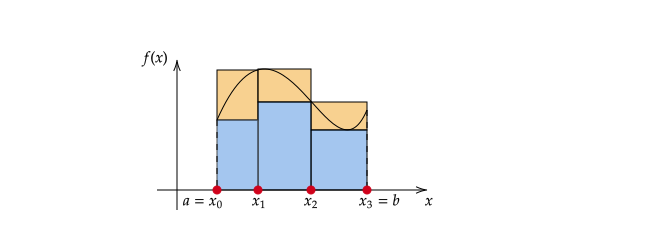
\includegraphics{riemannsums} 

}

\caption{The upper and lower Riemann sums for a function $f:[a,b] \to \mathbb{R}$ defined on a subdivision $P = \lbrace x_0,x_1,x_2,x_3 \rbrace$ of $[a,b]$. The lower Riemann sum is the total area of the blue rectangles, and the upper Riemann sum is the total area of the blue and orange rectangles.}\label{fig:Riemann}
\end{figure}

\hypertarget{refinements}{%
\subsubsection{Refinements}\label{refinements}}

At this stage, given a bounded function \(f:[a,b] \to \mathbb{R}\), we have a way of subdividing the domain and a way of estimating the area under \(f\). We'd now like to consider what happens to the estimates as we make our subdivision finer. This leads on to the idea of a refinement:

\BeginKnitrBlock{definition}[Refinement]
{\label{def:def4} }Let \(P = \lbrace x_0, x_1, \ldots, x_n \rbrace\) and \(Q = \lbrace y_0, y_1, \ldots, y_m \rbrace\) be subdivisions of \([a,b].\) Then \(Q\) is a \emph{refinement} of \(P\) if \(P\subseteq Q\).
\EndKnitrBlock{definition}
Note that under this definition, \(P\) is a refinement of itself!

\hypertarget{useful-results-for-subdivisions}{%
\subsection{Useful Results for Subdivisions}\label{useful-results-for-subdivisions}}

If we refine our subdivisions, what happens to the corresponding lower and upper Riemann sums? Luckily we have a set of results that tell us!

\BeginKnitrBlock{proposition}
{\label{prp:prop1} }Let \(f:[a,b] \to \mathbb{R}\) be bounded, and let \(P\) be a subdivision of \([a,b].\) Then:

\begin{itemize}
\tightlist
\item
  \(L(f,P) \leq U(f,P)\)
\item
  If \(Q\) is a refinement of \(P\), \[L(f,P) \leq L(f,Q)\;\; \text{and} \;\; U(f,Q) \leq U(f,P).\]
\item
  If \(R\) is \textbf{any} other subdivision, \[L(f,P) \leq U(f,R).\] (This says that every lower Riemann sum is smaller than every upper Riemann sum.)
\end{itemize}
\EndKnitrBlock{proposition}

The proofs of these results rely on some properties of suprema and infima, which are useful to know in any case!

\BeginKnitrBlock{proposition}
{\label{prp:prop2} }
Let \(\emptyset \neq S \subseteq T \subseteq \mathbb{R}\). Then

\begin{enumerate}
\def\labelenumi{\arabic{enumi}.}
\tightlist
\item
  \(\inf(S) \leq \sup(S).\)
\item
  \(\inf(S) \geq \inf(T)\) and \(\sup(S) \leq \sup(T).\)
\end{enumerate}
\EndKnitrBlock{proposition}

\hypertarget{the-definition}{%
\subsection{The Definition!}\label{the-definition}}

We're almost ready to define the (Riemann) integral! For our bounded function \(f:[a,b]\to\mathbb{R}\), the set of all lower sums is bounded above, and the set of all upper sums is bounded below. Therefore, we can talk about their supremum and infimum respectively. These have special names, and are correspondingly known as \emph{lower and upper Riemann integrals}.

\BeginKnitrBlock{definition}[Lower and Upper Riemann Integrals]
{\label{def:def5} }Let \(f:[a,b] \to \mathbb{R}\) be bounded. Then:

\begin{itemize}
\tightlist
\item
  The \emph{lower Riemann integral} is \[\underline{\int_a^b} f := \sup\left\lbrace L(f,P) \bigg\lvert\; \text{$P$ is a subdivision of $[a.b]$}\right\rbrace.\]
\item
  The \emph{upper Riemann integral} is \[\overline{\int_a^b} f := \inf\left\lbrace U(f,P) \bigg\lvert\; \text{$P$ is a subdivision of $[a.b]$}\right\rbrace.\]
\end{itemize}
\EndKnitrBlock{definition}

And now, after much ado, we can finally say what it means for a function to be Riemann integrable!

\BeginKnitrBlock{definition}[Riemann Integral]
{\label{def:def6} }Let \(f:[a,b] \to \mathbb{R}\) be bounded. Then \(f\) is \emph{Riemann integrable} if \[\underline{\int_a^b} f = \overline{\int_a^b} f.\] If this happens, then the (Riemann) integral of \(f\) is defined to be the common value, and given the notation \(\int_{a}^b f.\)
\EndKnitrBlock{definition}

\hypertarget{hints}{%
\section{Hints}\label{hints}}

As per usual, here's where you'll find the problem sheet hints!

\begin{enumerate}
\def\labelenumi{\arabic{enumi})}
\tightlist
\item
  Have a look back at the example we did in tutorials --- this one is pretty similar! Calculate both the lower and upper Riemann sums, and make sure to justify the main steps of your argument. Another thing, feel free to quote the values of \[\sum_{i=1}^{n} i^{k}, \quad k=0,1,2,\ldots\] as `standard results', although being able to prove them is good practice too!
\item
  First of all, this is an `if and only if', so there are two things to prove! The `\(\Leftarrow\)' direction should be fairly straightforward. For the `\(\Rightarrow\)' direction, what do you get from considering \(U(f,P) - L(f,P)\)?
\item
  Try the function \[h:[0,1] \to \mathbb{R}, \quad h(x) = xf(x),\] where \(f\) is as given in the question. Make sure to prove continuity at zero first. To prove that \(h\) is not integrable, show that the lower and upper Riemann integrals cannot be the same. For any subdivision \(P\), finding \(L(h,P)\) should be OK. For \(U(h,P)\), try and compare it to an upper Riemann sum of a function that you know the integral of.
\end{enumerate}

\end{document}
